% \documentclass[12pt]{scrreprt}
\documentclass[12pt]{report} 

% language may be romanian or english (default is english)
% type may be bachelor or master (default is bachelor)
\usepackage[language=english, type=bachelor]{style}
\usepackage{graphicx}   % for images
\usepackage{caption}    % for captionof

%\geometry{a4paper,top=2.5cm,left=3cm,right=2.5cm,bottom=2.5cm}
%in style
%controlling the appearance of your headers and footers
\usepackage{fancyhdr}
\pagestyle{fancy}
\lhead{}
\chead{}
\renewcommand{\headrulewidth}{0.2pt}
\renewcommand{\footrulewidth}{0.2pt}

\hypersetup{hidelinks}

\begin{document}

\specialization{INFORMATICĂ ENGLEZĂ}	
\title{Doclane}					   
\author{Robert Béres}											
\supervisor{Lect. PETRESCU Manuela}				
				
\maketitle


\newpage
\thispagestyle{empty}
\mbox{}
\newpage
\pagenumbering{roman} 

\cleardoublepage
ABSTRACT
\vspace{0.5cm}	
\hrule
\vspace{0.5cm}	
%\cleardoublepage

Doclane is a web application that helps citizens interact with public institutions without needing to visit in person multiple times. In many countries, including Romania, people still need to go to offices, wait in lines, and bring printed documents. This takes a lot of time and effort.

The problem is that most current systems are not fully digital, or they only cover part of the process. Some systems allow document submission but not tracking or feedback. Others work only for one institution.

Doclane tries to fix this by letting users submit requests online, upload documents, and see the status of their application. Employees at the institution can review the documents and send feedback if something is wrong or missing. This way, users do not need to visit in person just to find out that a document they provided is missing something.

The system is built as a web application using Go for the backend and Next.js for the frontend. It is fully cloud-native and scalable, adhering to modern best practices.

The thesis also looks at existing systems like GOV.UK, Enter Finland, and DocuSign. These systems solve parts of the problem but not all of it. Doclane tries to bring these ideas together in one system that can work across different institutions.

Doclane does not replace the physical pickup of final documents, since some documents require this by law. But it removes most of the unnecessary visits that happen before that step, which is where most of the time and frustration comes from.
\tableofcontents


\newpage
\pagenumbering{arabic}

\chapter{Introduction}

%\chapter*{Introducere}
\label{intro}

\section{Introducing the problem}

\par Public institutions play an important role in the daily lives of citizens, providing access to services such as official documents, permits, and administrative procedures. Because of this, it is important that the processes involved are efficient, reliable, and easy to use.

\par In many cases, these processes are still based on physical documents and in-person interactions. Citizens are often required to visit institutions, wait in queues, and submit printed files in order to complete simple requests. This approach leads to long waiting times, repeated visits, and inefficient handling of information.

\par In addition, physical documents can be lost, damaged, or incorrectly processed, which can delay important procedures. These inefficiencies do not only create inconvenience, but can also impact the ability of citizens to complete time-sensitive administrative tasks.

\par As a result, improving the way public institutions handle document-based workflows becomes an important problem to address.

\section{Role of Information Technology in Public Administration}

\par The use of information technology in public institutions has become increasingly important in recent years. Digital systems allow institutions to manage large amounts of data, automate processes, and reduce the time required to complete administrative tasks.

\par By moving services to digital platforms, interactions between citizens and institutions can be simplified. Instead of relying on physical documents and in-person visits, many processes can be handled online, improving accessibility and reducing waiting times.

\par In addition, digital systems make it easier to store, organize, and retrieve information. This can improve decision-making and reduce errors caused by manual processing of documents.

\par However, the adoption of such systems is not always straightforward. Public institutions may face challenges such as limited financial resources, lack of technical infrastructure, and insufficient digital skills among both employees and citizens.

\par Despite these challenges, the use of information technology remains a key factor in improving the efficiency and quality of public services.

\section{Challenges in Traditional Systems}

\par Traditional document handling in public institutions comes with several practical challenges that affect both citizens and employees.

\par One of the main issues is the need for physical presence. In most cases, citizens are required to visit an institution in person in order to submit or collect documents. This creates queues and waiting times, especially during busy hours or peak periods.

\par Another problem is the use of paper-based documents. Files are printed, copied, and stored physically. This takes space and also creates the risk of documents being lost, damaged, or misplaced. It also makes it harder to search and manage information when needed.

\par The process of checking and validating documents is often manual. Employees need to go through each file one by one, which takes time and can lead to delays, especially when the number of requests is high.

\par Feedback to citizens is also not always immediate. If a document is missing or incorrect, the citizen usually finds out later, sometimes after waiting for a long time or making another visit. This leads to repeated submissions and additional waiting time.

\par In addition, many of these processes are not transparent to the user. Citizens often do not know the current status of their request or how long it will take until it is completed.

\par These challenges show that the traditional way of handling document-based workflows is slow and can be improved with more structured and digital solutions.

\section{Limitations of existing digital solutions}

\par Even though some public services already use digital platforms, they are often limited in scope. Most of these systems are built for a specific type of service or a single institution.

\par In many cases, users still need to switch between different systems depending on the service they need. This creates fragmentation and makes the overall process less consistent.

\par Some systems also only cover part of the workflow, such as submitting documents or signing them, but not the full process from submission to final approval and feedback.

\par Because of this, there is still a need for systems that can be reused across different institutions, where each institution can use its own instance of the same workflow structure instead of relying on completely separate tools.

\section{Proposed solution}

\par The proposed system, Doclane, is a web-based application designed to handle document-based workflows between citizens and public institutions.

\par The system allows users to submit requests, upload required documents, and track the status of their applications. On the other side, institution employees can review submissions, validate documents, and provide feedback when needed.

\par The goal of the system is to reduce the need for physical visits and repeated submissions by moving the process into a structured digital workflow.

\par Doclane also focuses on making the process more clear for users by showing what is required at each step and giving feedback when something is missing or incorrect.

\section{Objectives}

\par The main objective of this thesis is to design and implement a system that improves document-based workflows in public institutions.

\par The specific objectives include:
\begin{itemize}
    \item Designing a backend system that can handle document requests.
    \item Implementing secure authentication and role-based access.
    \item Building a structured workflow for submission and validation.
    \item Using cloud storage for document handling.
    \item Making the system scalable and easy to extend.
\end{itemize}

\section{Scope of the system}

\par The system focuses on improving the workflow between citizens and public institutions when it comes to document-based requests.

\par It does not change the legal process of document approval. Final decisions are still made by authorized personnel within the institution.

\par The system is designed as a support tool that helps organize and digitalize the existing workflow, not replace institutional rules or procedures.

% \section{Motivation}

% \par The idea behind Doclane was optimizing a complex, lengthy process that most people go through on a regular basis into a predominantly digital, simplified and shorter one.

% \par With the way public institutions are structured, they handle thousands of requests per day, many of those requiring files that will be kept in a physical archive for years, or maybe indefinetly. This is not only wasteful when taking into account the consumed paper, but also in human time.

% \par Paper can be lost and it can be damaged. The solution to making sure it won't get lost is to make copies of it, which is again wasteful. Why not optimize this process by digitalizing the biggest bottleneck in it and implement modern technologies such as cloud storage, which proves to be so much more efficient in the long term? And why stop at just cloud storage, when we can optimize this process, to also save time instead of physical resources? We reduce costs, save the planet and save our time, everyone wins in this equation.

% \section{Problem statement}

% \par This thesis addresses inefficiencies in traditional public administration workflows, particularly in the submission, validation, and processing of document-based requests. These workflows are often characterized by manual handling, repeated physical interactions, and lack of structured feedback mechanisms.

% \section{Objectives}

% The main objective \cite{Sommerville2010} of this thesis is to design and implement a cloud-based system that improves the efficiency of document request workflows in public institutions.

% The specific objectives include:
% \begin{itemize}
%     \item Designing a scalable backend architecture for handling document requests.
%     \item Implementing secure authentication and role-based access control.
%     \item Providing a structured document submission and validation workflow.
%     \item Integrating cloud storage for secure file management.
%     \item Ensuring system reliability through modern cloud infrastructure.
% \end{itemize}

% \section{Limitations}

% The system is designed as a digital workflow optimization platform and does not replace the legal authority of public institutions. Final document issuance and validation remain under institutional control.

% \section{Current process}

% \par Let's take the example of how you could, in this current day, retrieve a document from a public institution, maybe an urbanim certificate so that you can build stuff on your property. You'd schedule an appointment whenever the next free time slot is (and queue times are definetly not short), then you go present yourself, you take your identification with you and all the required documents such that it can be emitted. Let's say you did not forget anything and you do not need to reschedule, although this happens sometimes too. By the time you have your certificate emitted, half your day is gone, not only because the process itself is lengthy but due to the sheer number of other citizens that need their requests solved you might have to wait longer than your appointment timeline, and maybe delays occur too.

% \section{What Doclane promises}

% \par Doclane digitalizes the bottleneck in this entire process. Let's take a look at how you can receive the same urbanism certificate while reducing human interaction to just one step. You wake up, you log in to Doclane, your account is linked to the local institution you belong to, and in the app you select the certificate you need, and then choose to submit the request. You will be prompted by the application to upload relevant documents to your applications in specific slots, each slot also providing you with examples on how the uploads should look. You uploaded everything within 5 minutes, then on the other side public institution employees are notified, they check the documents, emit an approval and you go pick up your document.

% \par Did you submit something that the institution cannot accept? They can notify you within the application and let you know what you didn't do right, so that you may correct it. No more re-scheduling appointments and losing hours upon hours to have the paper you need released.
\chapter{Related work}
\label{chap:ch2}

\par This chapter presents existing systems and research related to digital document handling and public administration workflows. The goal is to show how similar problems have been handled in other systems and what solutions already exist.

\par The systems and studies presented here focus on document submission, electronic workflows, and online public services. Some of them are real systems used by governments, while others are research papers that propose ways to improve administrative processes.

\par After presenting these systems, a short comparison is made to identify their limitations in relation to the problem addressed by this thesis. This helps explain the motivation behind Doclane and how it differs from existing solutions.

% -------------------------------------------------

\section{Automated electronic document management systems in municipal units}

Koptyakova et al. \cite{koptyakova2019} present a system for automated electronic document management in municipal institutions. The paper focuses on improving how public institutions handle documents and reducing the time needed for administrative work.

The authors explain that traditional document workflows in municipal units are slow and depend on manual work. Documents are usually registered, tracked, and processed by hand, which can cause delays when the number of requests is high.

To solve this, the paper proposes an automated system that digitizes document registration, tracking, and processing inside municipal institutions. This reduces manual work and makes the process faster.

The study also looks at the cost and benefits of such systems. It mentions that the payback period can be short because less manual work is needed and efficiency increases.

However, the system is mainly used inside one municipal institution. It focuses on internal document handling and not on the full process between citizens and institutions.

Compared to this, Doclane focuses on the full workflow between citizens and public institutions, including submission, validation, and feedback.

% -------------------------------------------------

\section{Digital document systems in public sector implementation}

Az Ab Aziz et al. \cite{abaziz2019ddms} study the implementation of a Digital Document Management System (DDMS) in the Malaysian public sector. The system is used to manage documents and records inside government institutions and aims to reduce paper use and improve document handling.

The paper shows that even when such systems exist, adoption is not always high. The main issues are not only technical, but also related to policy, training, security, and internal support.

The authors explain that successful implementation depends on clear guidelines and coordination between agencies. Without this, different institutions use the system in different ways, which reduces its effectiveness.

Compared to this, Doclane focuses more on workflows between citizens and institutions, but the same idea applies: a system is only useful if it is properly adopted and used in real work.

% -------------------------------------------------


\section{Document Management Systems in Public Sector Integration}

Electronic document management systems in public sector institutions are often part of larger information systems. International Journal of Advances in Engineering \& Technology \cite{dms_integration_2012} explains that government institutions use many systems such as finance systems, HR systems, CRM systems, and web portals. Because of this, document management systems need to work with other systems.

The authors explain that integration means systems can exchange data and work together, not that they are merged into one system. This is important because many public sector processes depend on data moving between systems.

The study also shows that integration can improve efficiency by reducing manual work and making workflows simpler. However, it is not easy. It can be expensive, take time, and may require changes in several systems. Some integration projects also fail due to poor planning.

Even with these problems, integration is still needed if institutions want to improve digital workflows.

Compared to this, Doclane also follows the idea of integration by connecting document workflows with different parts of an administrative system and improving communication between users and institutions.

% -------------------------------------------------

\section{Enter Finland}

Enter Finland (\url{https://enterfinland.fi}) is a government service used in Finland for immigration applications. Users can fill forms online, upload documents, and pay fees. After submission, some cases still require an in-person visit.

The system reduces the need for paper submission and physical visits at the start of the process. However, it is limited to immigration services and one type of institution.

Compared to this, Doclane is designed for different types of document workflows across multiple institutions.

% -------------------------------------------------

\section{DocuSign}

DocuSign (\url{https://www.docusign.com}) is a platform used for signing documents online. Users can upload documents, send them for signature, and track their status.

It removes the need to print and scan documents in many cases. It is mostly used in business environments.

However, it focuses mainly on signing and approval. It does not support full administrative workflows like structured requests or multi-step validation.

Compared to this, Doclane handles full workflows from submission to approval and feedback.

% -------------------------------------------------

\section{GOV.UK Services}

GOV.UK (\url{https://www.gov.uk}) is a UK government platform for online public services. Users can apply for documents, submit forms, and access different services.

It reduces the need for physical visits and allows many tasks to be done online. It covers many services in one platform.

However, each service has its own workflow and is not part of one unified system.

Compared to this, Doclane aims to provide a single workflow system for different types of document requests.

% -------------------------------------------------

\section{Comparison}

The systems described above solve parts of the same problem in different ways.

Enter Finland is focused on one domain. GOV.UK provides many services, but they are separate. DocuSign focuses on document signing.

All of them reduce paper use and improve digital access, but they are limited either by domain, structure, or function.

% -------------------------------------------------

\section{Gap}

There is no widely used system that handles document-based workflows across multiple public institutions in one unified system.

Most systems are either domain-specific, split into separate services, or focused on one function like signing.

Doclane addresses this by providing a unified workflow for submission, validation, feedback, and approval across institutions.
\chapter{Implementation}
\label{chap:ch3}

\par The backend of Doclane is written in Go, and the frontend is built with Next.js. Go was chosen because it is fast, has a large standard library, and handles errors in a way that makes bugs easier to track. Next.js was chosen because Doclane is a dynamic application that makes many requests to the backend, and server-side rendering helps keep loading times short.

\begin{center}
    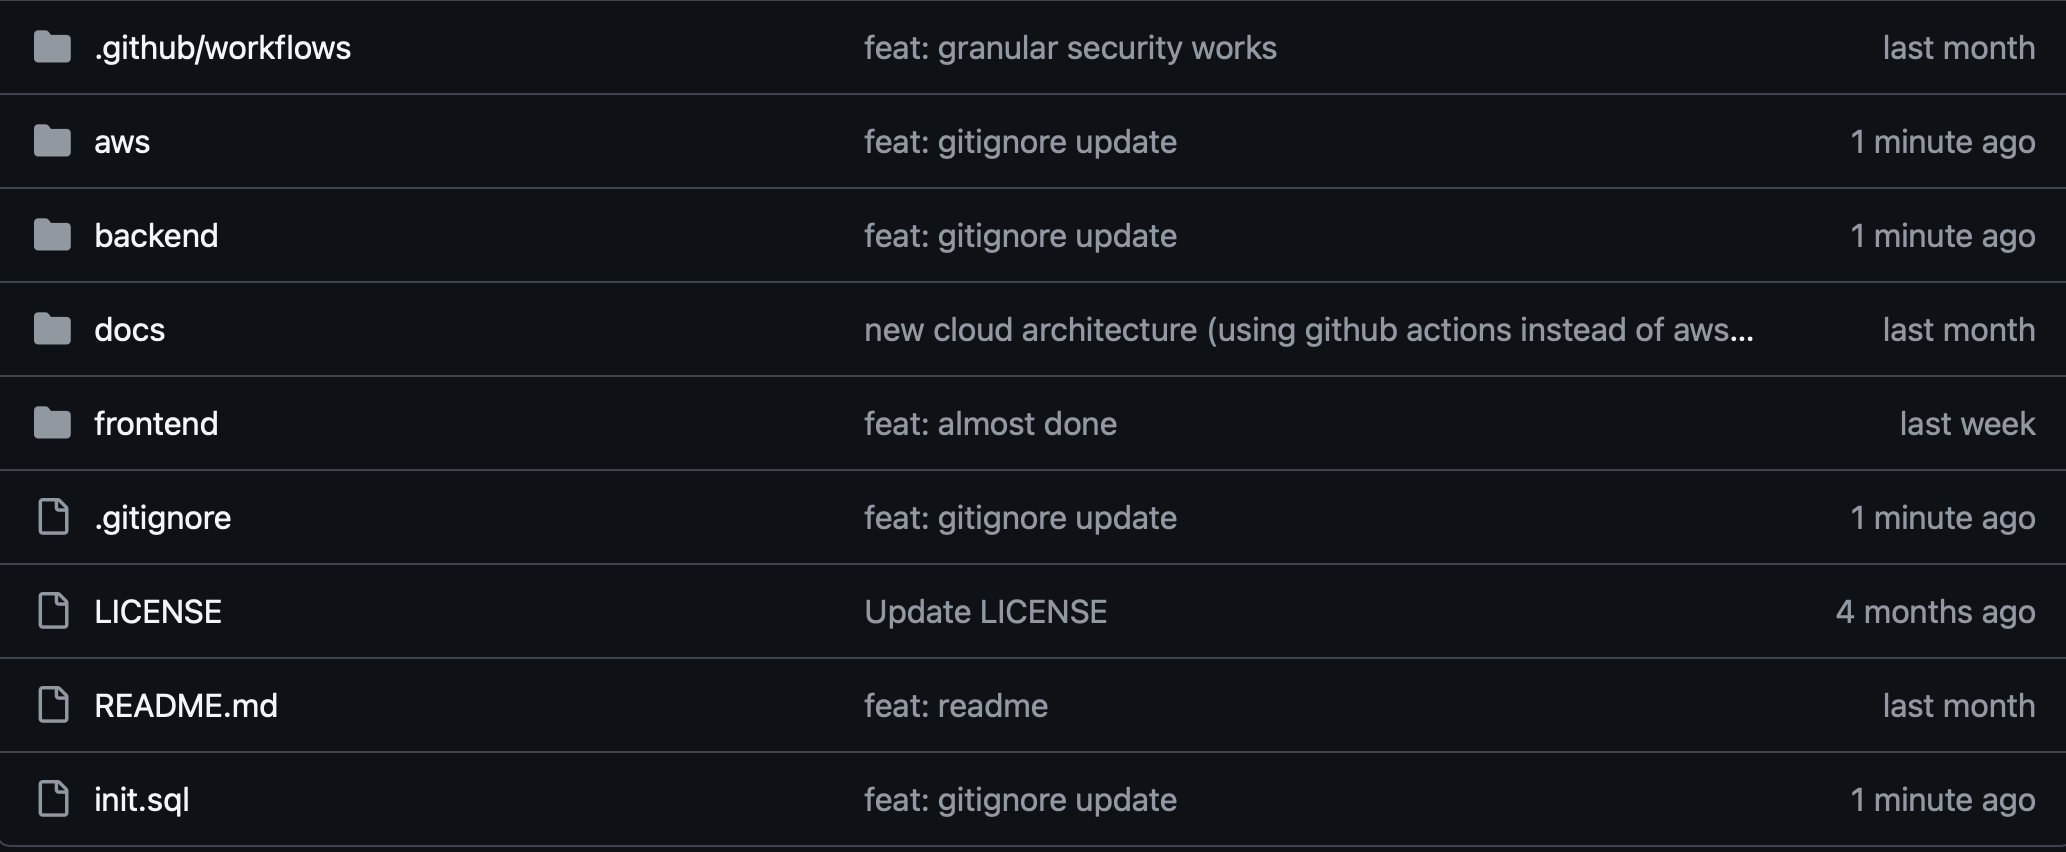
\includegraphics[width=0.8\textwidth]{figures/folder-structure.png}
    \captionsetup{type=figure}
    \captionof{figure}{Overview of Doclane's folder structure.}
\end{center}

\section{Backend}

\subsection{Go}

\par Go is a statically typed, compiled programming language. It has a simple syntax and a standard library that covers most common needs. It is also fast to write and produces efficient binaries.

\subsection{Layers}

\par The backend code is split into four layers:

\begin{itemize}
    \item Handler layer: handles incoming HTTP requests and extracts the needed information from them, such as JWT claims, resource IDs, or uploaded files.
    \item Service layer: contains the business logic and validations. For example, it checks whether a user has the right role to perform an action. A user cannot view the files of a request unless they are an admin or they belong to the department that manages that request.
    \item Repository layer: executes queries on the database. It trusts everything passed to it, since all validation happens in the service layer. Transactions are used when multiple database operations need to succeed together for an action to be considered complete.
    \item Model layer: holds the data structures used across the application, such as users, requests, templates, invitation codes, and comments. DTOs (Data Transfer Objects) are used in some cases to enrich data from the database. For example, when retrieving a request, the DTO also includes the requester's name and email, not just their ID.
\end{itemize}

\subsection{Authentication}

\par Authentication is handled using JWTs (JSON Web Tokens) issued by AWS Cognito. A JWT is a stateless token that contains information about the user such as their ID, role, department, and name. The information inside the token is readable by anyone, but it cannot be changed without the signature becoming invalid. The backend rejects any token with an invalid signature.

\par The token is stored in an HTTP-only cookie. This means JavaScript running in the browser cannot access it, which protects against XSS (Cross-Site Scripting) attacks. More details about Cognito and how it is configured are in chapter 4.

\subsection{API Response}

\par Every response from the API follows the same structure. This makes it easier for the frontend to handle responses in a consistent way. Every response contains:

\begin{itemize}
    \item \textbf{success} - a boolean that says whether the request worked or not.
    \item \textbf{message} - optional, a short description of what happened.
    \item \textbf{error} - optional, an error message present when success is false.
    \item \textbf{data} - optional, contains any data returned by the request.
\end{itemize}

\begin{center}
    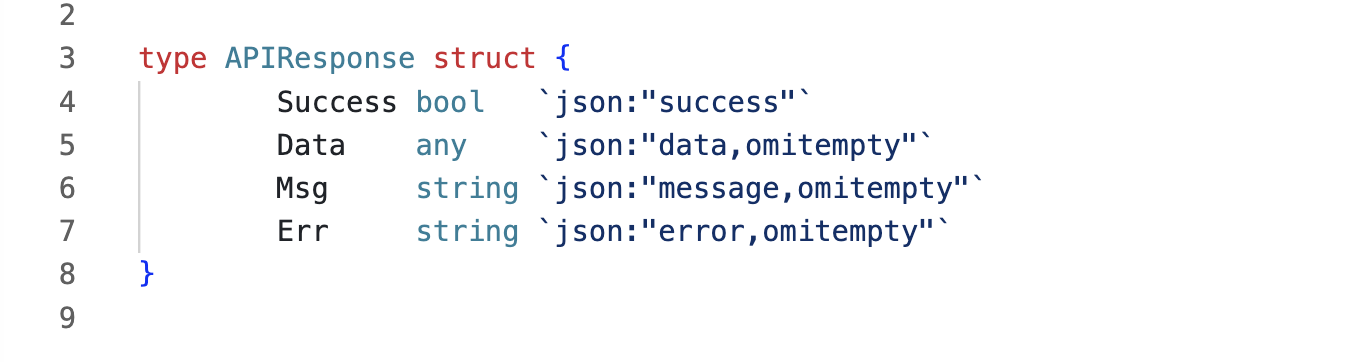
\includegraphics[width=0.8\textwidth]{figures/api-response.png}
    \captionsetup{type=figure}
    \captionof{figure}{API Response struct.}
\end{center}

\subsection{Custom Errors}

\par Custom error types are defined and used across the backend. This gives a unified way to handle errors and makes the code easier to read.

\subsection{Configuration}

\par There is a single configuration file that acts as the main setup for the application. It is where all service and repository instances are created and exported. If a repository implementation needs to be changed, only this file needs to be updated. Everything else continues to work without changes.

\subsection{Middleware}

\par Most routes in the application are protected by middleware. The middleware checks that every incoming request has a valid JWT token before it reaches the handler. Requests with missing or invalid tokens are rejected early.

\par There are two middleware checks in Doclane. The first checks that the token is valid and was signed correctly by Cognito. The second checks that the user account is active.

\subsection{File Storage}

\par Uploaded files are stored in S3, which is a file storage service from AWS. The file storage logic is separated from the rest of the application so the app does not depend on it directly. All file access is done through presigned URLs, which are temporary links that give access to a specific file for a limited time. More details about S3 and how it is set up are in chapter 4.

\subsection{Routing}

\par Backend routing is done using the Chi library, which is a third party Go package. Although Go's standard library handles many things well, HTTP routing is an area where external help is useful. Chi makes it easy to organize routes in a clear and readable way.

\begin{center}
    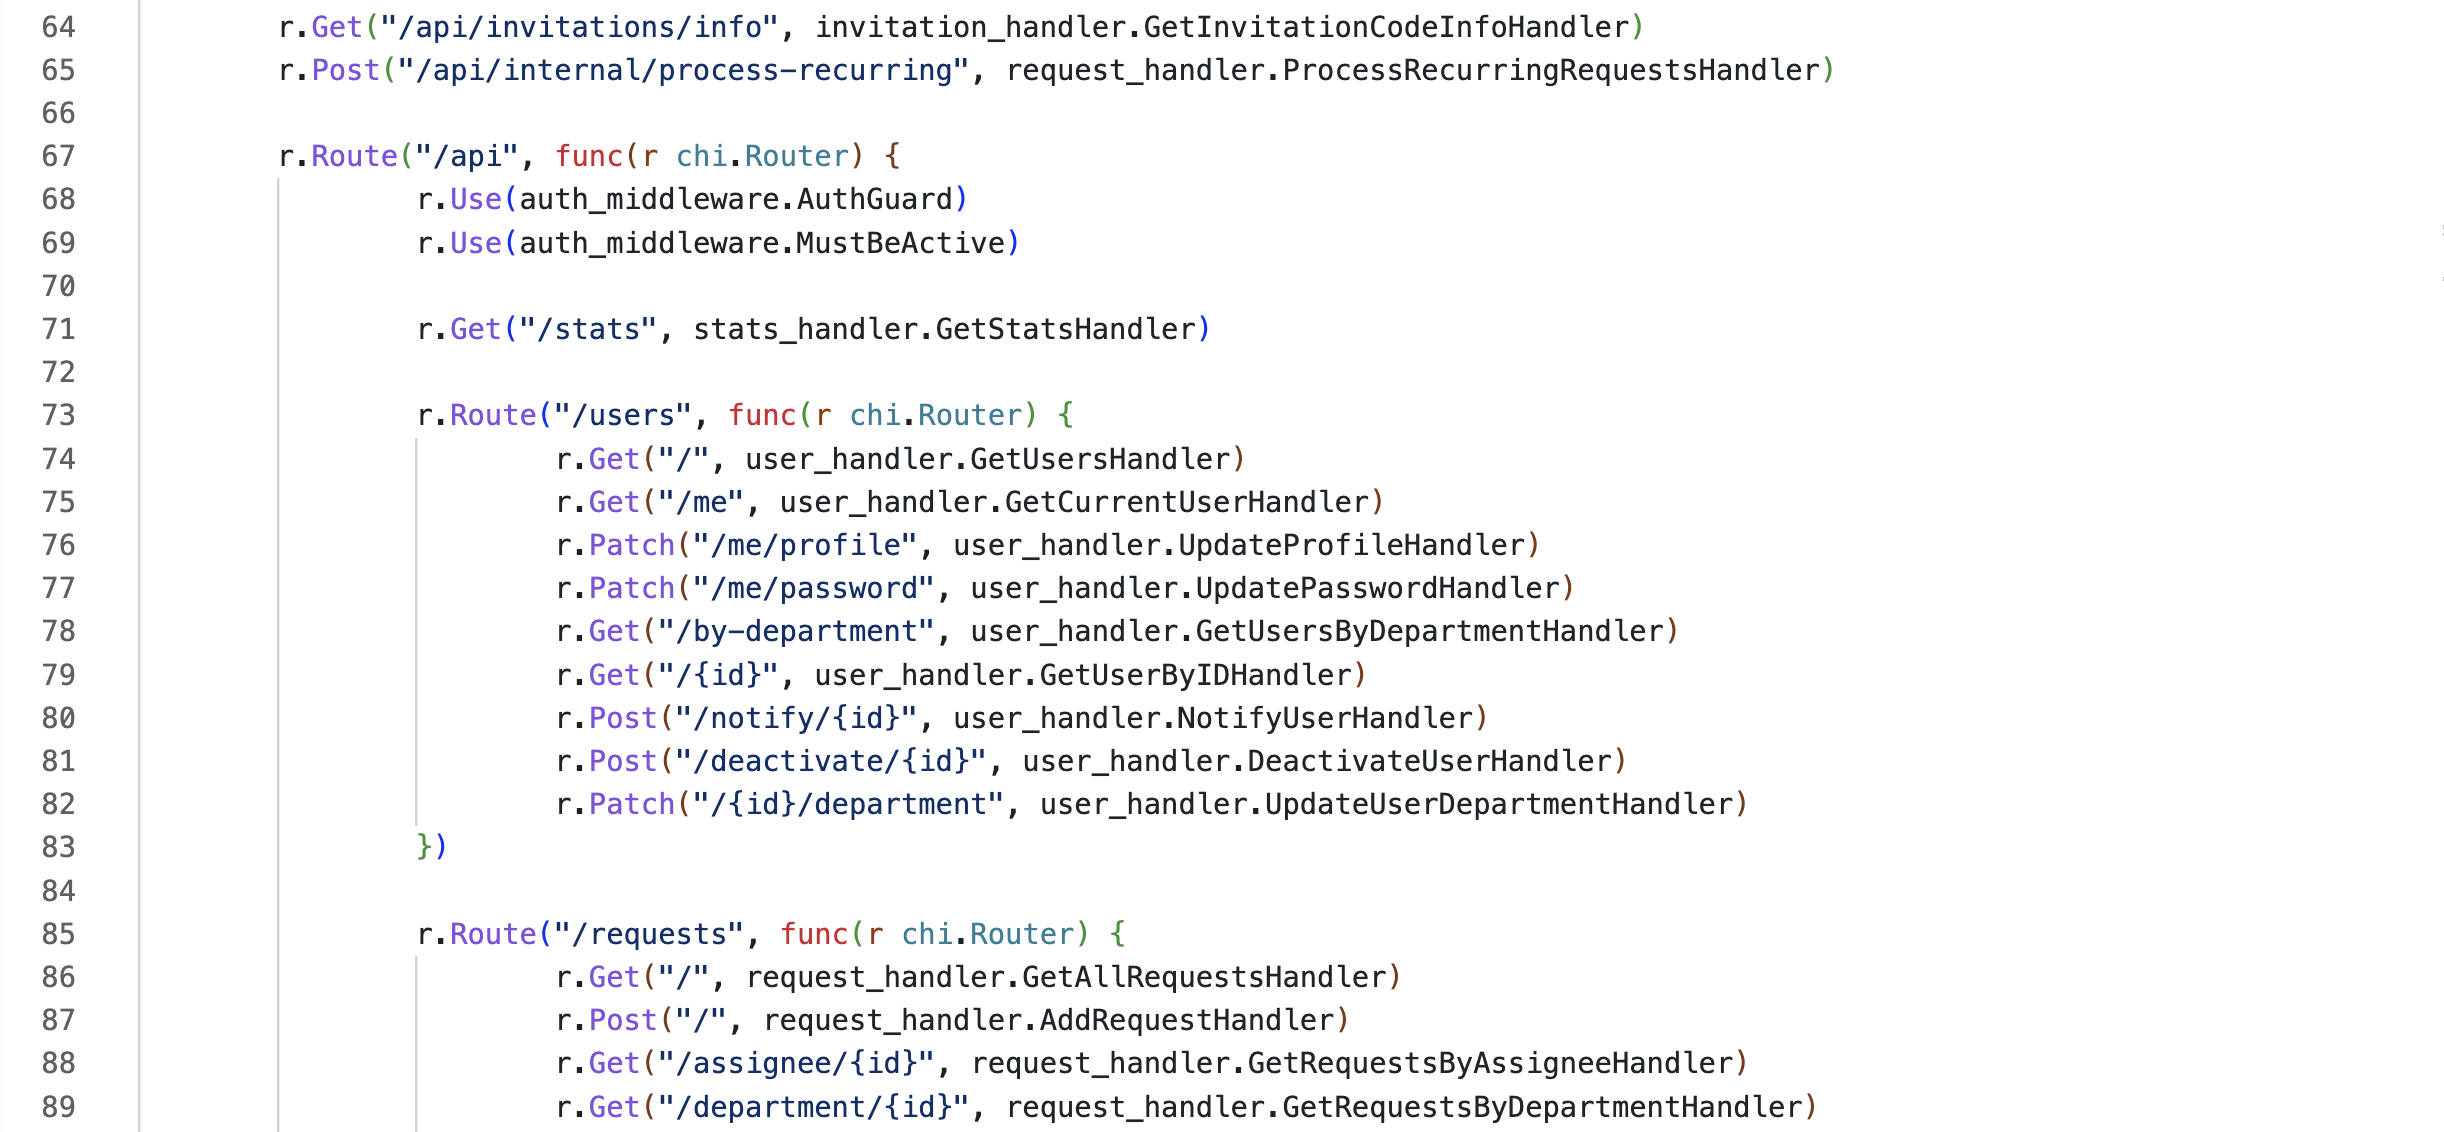
\includegraphics[width=0.8\textwidth]{figures/implementation/backend/chi-routes.png}
    \captionsetup{type=figure}
    \captionof{figure}{Routing for the backend.}
\end{center}

\section{Database}

\par PostgreSQL was chosen as the database engine. It is one of the most widely used relational databases and it fits the needs of Doclane well since the data has clear relationships between tables.

\begin{center}
    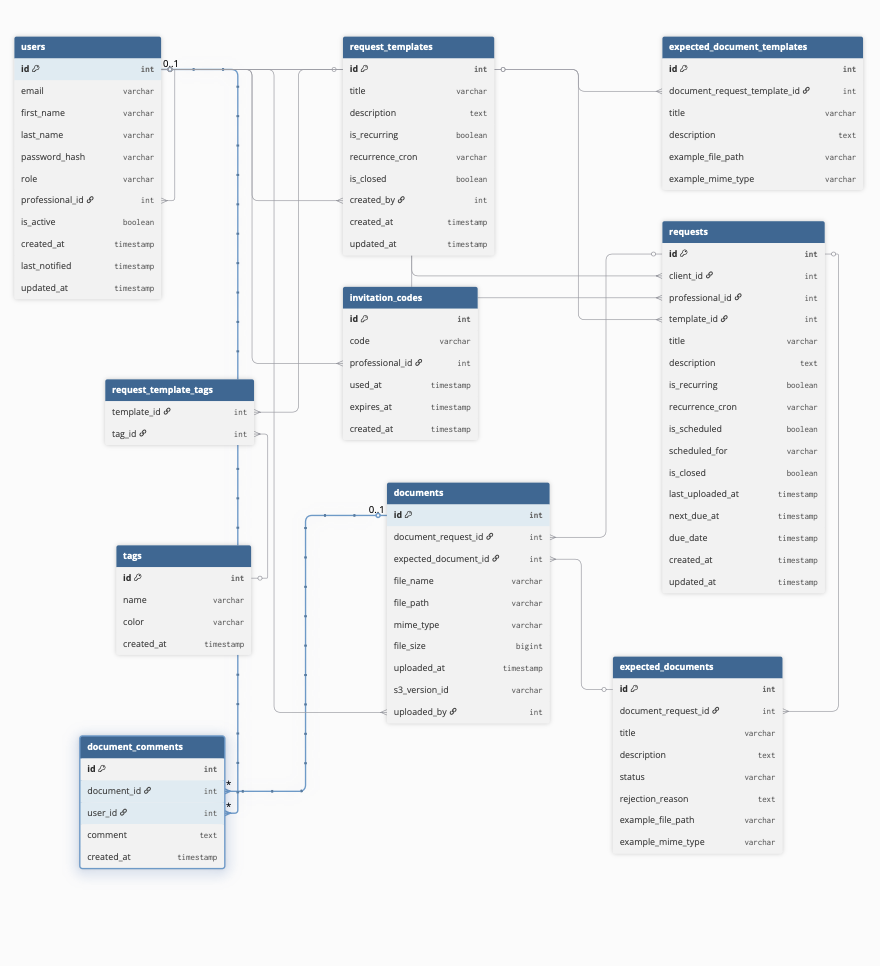
\includegraphics[width=0.8\textwidth]{figures/implementation/backend/database-diagram.png}
    \captionsetup{type=figure}
    \captionof{figure}{Database schema overview.}
\end{center}

\section{Frontend}

\par The frontend is built with Next.js, which is an open-source web framework built on top of React. It supports server-side rendering, which means pages can be prepared on the server before being sent to the browser.

\par Next.js was chosen because Doclane makes many requests to the backend on almost every page. If a client-side only framework like plain React was used, users would spend a lot of time on loading screens. With Next.js, data is fetched on the server before the page is shown, so the experience is faster.

\par Frontend code is split into small reusable components so that the same piece of UI does not need to be written more than once. This follows the DRY (Don't Repeat Yourself) principle, which is also applied in the backend but is most visible in the frontend.
\chapter{Deployment}
\label{chap:ch4}

\par When it comes to deploying an application, there are many paths one could take. One might be ordering a physical server at home and running your application on there, another one could be running it locally on your machine where only people in your network can access it, and another one could be deploying the application in the cloud. The last one was chosen for Doclane.

\section{Cloud computing}

\par Cloud computing was preferred since it is the more modern approach, and reduces overhead with managing physical servers. Without the burden and expenses of buying, setting up and maintaining servers, more effort could be redirected to the development of the app and adding features that bring more value to it. It is also that renting those servers means you can just get rid of them whenever you're not using them anymore, and you only pay for how much you use them.

\section{Amazon Web Services}

\par The deployment of the app was done on AWS. The architecture leverages containers orchestrated by Kubernetes, specifically the managed EKS (Elastic Kubernetes Service) offering from AWS.

\par AWS is the leading cloud provider, covering roughly 31\% of the global market as of 2026. Part of the reason it is so widely used is because it was the first to market, so it had the most amount of time out of all competitors to refine their services and offerings, which is half of the reason it was chosen. The other half was because the author of this thesis project is a certified Solutions Architect Professional on AWS and had a bias to pick this provider.

\subsection{Containers and Kubernetes}

\par A container is a lightweight, standalone package that includes everything needed to run a piece of software: the code, runtime, libraries and dependencies. Unlike virtual machines, containers share the host operating system kernel, making them fast to start and efficient with resources.

\par Docker is the tool used to build these containers. The backend and frontend of Doclane each have a Dockerfile that defines how the container image is built. The backend produces a small static Go binary running on a minimal base image, while the frontend uses Next.js standalone output on a Node.js base image.

\par Kubernetes is an open-source container orchestration platform. It takes your containers and runs them across a cluster of machines, handling scaling, networking, health checks and restarts automatically. Instead of manually starting containers on servers, you declare what you want (for example: "run 2 copies of the backend") and Kubernetes makes it happen.

\par EKS (Elastic Kubernetes Service) is AWS' managed Kubernetes offering. AWS handles the control plane (the brain of the cluster), while you manage the worker nodes (the machines that actually run your containers). This removes the operational burden of maintaining Kubernetes itself while giving full access to its features.

\section{The architecture}

\par The architecture consists of an EKS cluster running in a VPC with two availability zones. Traffic enters through an ALB (Application Load Balancer) that routes requests to the appropriate service: the backend or the frontend. The backend connects to an RDS PostgreSQL database and an S3 bucket for document storage. Authentication is handled by Cognito.

\subsection{Networking}

\par The networking part of Doclane consists of a VPC (Virtual Private Cloud) in the eu-west-1 Region on AWS. This VPC consists of two private subnets and two public subnets. The private subnets host the EKS worker nodes and the RDS database, so that no direct public internet access can be established to them.

\par The public subnets host the NAT Gateway and the ALB (Application Load Balancer). The NAT Gateway allows resources in private subnets to reach the internet (for example to pull container images) without being directly accessible from the internet.

\par Both the private and public subnets span two AZs (Availability Zones), such that high availability is achieved. In case one data center from AWS goes down where our application runs, then it will still continue to run as if nothing has happened.

\par An internet gateway was provisioned and added to the route table of the public subnet, such that internet access is possible to and from it. Private subnets are associated with a route table that routes internet-bound traffic through the NAT Gateway. So the thing that makes a subnet public or private is whether or not the associated route table has a direct route to the internet gateway or goes through a NAT Gateway.

\par The subnets are tagged with Kubernetes-specific labels so that the AWS Load Balancer Controller can automatically discover which subnets to place ALBs in.

\subsubsection{Security}

\par When it comes to network security, the architecture leverages Security Groups for securing traffic at the pod level and at the RDS level.

\par A Security Group in AWS is a stateful firewall that operates at a single resource level. It consists of inbound / outbound rules, inbound rules meaning what kind of traffic is allowed (on which port and from which source), while outbound rules control what traffic is allowed to go out of our resource.

\par The RDS database is protected by a Security Group that only allows inbound traffic on port 5432 from the EKS cluster Security Group. This means only pods running in the cluster can reach the database. Any other traffic is dropped.

\par The entire communication between the backend pods and RDS happens over encrypted connections (SSL/TLS is enforced on the database). Traffic between pods within the cluster uses the internal Kubernetes network and never leaves the VPC.

\subsection{Database layer}

\par RDS (Relational Database Service) was the preferred choice for the database. As a relational database was needed, the natural choice was AWS' managed service for this.

\par RDS is built in such a way that AWS handles all the operating system patching of the server that is running your database, and you also benefit from automated backups out of the box.

\par The engine is PostgreSQL, chosen for being popular, fast and well supported by RDS. The database schema is automatically applied on every fresh deployment by a Kubernetes Job that runs the initialization SQL script.

\subsection{Backend layer}

\par The backend runs as a Deployment in Kubernetes with 2 replicas by default. Each replica is a container running the Go binary that serves the chi HTTP router on port 8080. 

\par A HorizontalPodAutoscaler is configured to scale the backend from 2 to 6 replicas based on CPU utilization. If average CPU goes above 70\%, Kubernetes automatically adds more pods to handle the load.

\par Health checks are configured using Kubernetes liveness and readiness probes. The liveness probe ensures crashed containers get restarted. The readiness probe ensures traffic is only sent to pods that are ready to serve requests.

\subsubsection{IAM Roles for Service Accounts (IRSA)}

\par The backend pods need access to AWS services like S3, Textract, Bedrock, Polly and Cognito. Instead of using static credentials, the pods use IRSA (IAM Roles for Service Accounts).

\par IRSA works by linking a Kubernetes Service Account to an IAM Role. When a pod uses that Service Account, the AWS SDK automatically receives short-lived credentials scoped to exactly the permissions defined in the IAM Role. No static keys exist anywhere, not in the image, not in environment variables, not on disk.

\par The IAM policy attached to the backend pod role follows the principle of least privilege. It only allows the specific actions needed: uploading and downloading from the documents S3 bucket, calling Textract for text extraction, calling Bedrock for document interpretation, calling Polly for speech synthesis, and looking up users in Cognito.

\subsection{Frontend layer}

\par The frontend runs as a Deployment in Kubernetes with 2 replicas. Each replica runs the Next.js standalone server on port 3000. The standalone output mode produces a minimal server bundle that does not need the full node\_modules directory, keeping the container image small.

\par A HorizontalPodAutoscaler scales the frontend from 2 to 4 replicas based on CPU utilization.

\par Server-side rendering (SSR) calls from the frontend to the backend happen over the internal Kubernetes network using the service DNS name. This means SSR requests never leave the cluster and have minimal latency.

\subsection{Ingress and Load Balancing}

\par Traffic enters the cluster through an ALB (Application Load Balancer) that is automatically provisioned by the AWS Load Balancer Controller. This controller runs inside the cluster and watches for Ingress objects. When it sees one, it creates and configures a real ALB in AWS to match the routing rules defined in the Ingress.

\par The Ingress defines two routing rules: requests to /api are sent to the backend service, and all other requests are sent to the frontend service. The ALB terminates TLS using an ACM certificate and redirects HTTP traffic to HTTPS.

\par The ALB uses IP-mode target groups, meaning it routes traffic directly to pod IPs rather than going through node ports. This is more efficient and allows for faster health checks.

\subsection{DNS and HTTPS}

\par The application is served at thesis.robert-beres.com. An ACM (AWS Certificate Manager) certificate was provisioned for this domain and validated automatically via DNS. The certificate is attached to the ALB so all traffic is encrypted.

\par A Route53 alias record points the domain to the ALB. When the infrastructure is torn down and recreated, the ALB gets a new DNS name, but Terraform automatically updates the Route53 record to point to the new one.

\subsection{Document storage}

\par S3 (Simple Storage Service) is used for storing uploaded documents. The bucket has versioning enabled so previous versions of files are preserved, and server-side encryption is applied to all objects.

\par The backend generates presigned URLs for downloads. This means clients download directly from S3 using a temporary URL that expires after a set time, without any permanent credentials ever existing. This makes the process so much more secure since if somehow credentials get leaked the attack surface is very small due to the scoped permissions, and the attack surface is also ephemeral.

\subsection{Authentication}

\par Cognito is used as the identity provider. It manages user registration, login, password policies and token issuance. The frontend uses the Amplify library to interact with Cognito directly from the browser.

\par After a user logs in, Cognito issues a JWT (JSON Web Token). This token is stored in an HTTP-only cookie and sent with every request. The backend validates the token by checking its signature against Cognito's public keys (JWKS).

\subsection{Logging and monitoring}

\par Container logs from all pods are collected by Kubernetes and can be viewed using kubectl. The structured JSON logging from the backend makes it easy to filter and search for specific events or errors.

\section{Machine Learning}

\par This section goes into detail on the AWS services leveraged to build the machine learning assisted features aforementioned in the implementation chapter.

\subsection{Textract}

\par Textract is a fully managed serverless service offered by AWS that extracts text from documents. API calls are made to Textract from Doclane in order to extract text from documents.

\subsection{Polly}

\par Polly is a fully managed serverless service offered by AWS that generates speech from text. API calls are made to Polly to generate speech from selected documents.

\subsection{Bedrock}

\par Bedrock is a fully managed serverless service offered by AWS that gives you access to different LLMs that you can prompt. In our case we use the Nova Lite model from Amazon to interpret whether a document provided by an user is actually what it is required by the request.

\section{Infrastructure as Code - Terraform}

\par Whenever deploying applications in the Cloud, you can manually click in the AWS console and provision everything you need. It's straight forward, intuitive and it provides a friendly experience. Although this is convenient, it is a manual process. And manual processes are prone to errors. It becomes easy to forget what change in configuration you made last week, more simply put, it's a mess.

\par That's where the concept of IaC (Infrastructure as Code) comes into play. This involves specifying your infrastructure in a declarative manner, and having everything defined as code, it becomes much easier to maintain and have control over.

\par Terraform by HashiCorp is the chosen tool for the project. Unlike CloudFormation which is AWS-specific, Terraform is cloud-agnostic and has a large ecosystem of providers. It was chosen for its ergonomics: features like force\_destroy on S3 buckets, native Helm and Kubernetes providers, cross-region resource management with provider aliases, and the ability to manage the entire stack (AWS resources, Kubernetes manifests, Helm charts) from a single tool.

\subsection{State management}

\par Terraform keeps track of what it manages in a state file. This file maps the resources defined in code to the real resources in AWS. It is stored remotely in an S3 bucket with versioning enabled, so it can be recovered if corrupted. A DynamoDB table is used as a lock to prevent two people (or two CI runs) from modifying infrastructure at the same time.

\subsection{Stack layout}

\par The infrastructure is split into multiple Terraform stacks, each with its own state file:

\par \textbf{bootstrap} - Creates the S3 bucket and DynamoDB table for state management. Run once, never destroyed.

\par \textbf{platform-data} - Contains long-lived resources that are cheap to keep running: ECR container registries, Cognito user pool, ACM certificate, GitHub OIDC role. These persist across compute teardowns.

\par \textbf{platform-compute} - Contains the expensive resources: VPC, NAT Gateway, EKS cluster, RDS database, S3 documents bucket, IRSA roles. These are created when working and destroyed when not needed.

\par \textbf{workload} - Contains everything inside the Kubernetes cluster: Helm charts, deployments, services, ingress, database seeding jobs. Destroyed together with platform-compute.

\par This split allows tearing down the expensive compute resources while not using the app, since in development you do not need the app running 24 hours a day, while keeping the cheap persistent resources alive. A full environment can be recreated from scratch with a single command.

\subsection{Ephemeral environments}

\par The entire compute layer is designed to be ephemeral. Running \texttt{make up} provisions the full environment from scratch in about 15 minutes: VPC, NAT, EKS cluster, RDS database, container deployments, database schema seeding, admin user creation, ALB, HTTPS, DNS record. Running \texttt{make down} destroys everything in about 10 minutes, bringing the cost to zero.

\par This is possible because:
\begin{itemize}
    \item Container images persist in ECR between sessions
    \item The Cognito user pool persists so users do not need to re-register
    \item The ACM certificate persists so DNS validation does not need to happen again
    \item The database schema is applied automatically by a Kubernetes Job on every fresh deployment
    \item The admin user is bootstrapped automatically by another Kubernetes Job
\end{itemize}

\section{Continuous Integration / Continuous Deployment}

\par Modern practices of deployment have been adopted, such that the deployment pipeline of the application is fully automated. Once changes are pushed to the main branch, container images are automatically built and pushed to ECR.

\par CI/CD has been done with the help of GitHub Actions. GitHub Actions are convenient to use when your repository is already on GitHub, hence why they were chosen.

\par The pipeline builds Docker images for the backend and frontend, tags them with the git commit SHA for traceability, and pushes them to ECR. The backend and frontend are built independently, only when their respective code changes.

\par Updates happen leveraging the least-privilege principle, without any permanent credentials ever existing or being stored anywhere. The GitHub Action worker generates an ID token using GitHub's OIDC (OpenID Connect). GitHub signs this token with their private key, and this signed token is then passed to AWS to prove the identity of the runner.

\par In AWS, an OIDC provider is configured in IAM, trusting GitHub and allowing Role Assumptions for the worker as long as it proves it's from the Doclane repository. The IAM role assumed by the worker only has permissions to push images to the two ECR repositories. Nothing else.

\par Role Assumption in AWS is a concept that allows generating temporary credentials to perform actions in an AWS account, leveraging the STS (Secure Token Service) from AWS. Credentials are short-lived. Once the credentials expire they cannot be used anymore, and even if they somehow get leaked the damage would be minimal since the only thing they allow is pushing container images.

\section{Containerization}

\par Both the backend and frontend are packaged as Docker containers using multi-stage builds.

\subsection{Backend container}

\par The backend Dockerfile uses a two-stage build. The first stage uses the Go compiler to build a fully static binary with no external dependencies. The second stage uses a minimal distroless base image that contains no shell, no package manager, nothing except the binary and CA certificates. The final image is about 36 MB and runs as a non-root user.

\subsection{Frontend container}

\par The frontend Dockerfile also uses a multi-stage build. The first stage installs dependencies and runs the Next.js build. The second stage copies only the standalone output (a minimal server bundle) into a Node.js Alpine image. The final image is about 370 MB and runs as a non-root user.

\par The NEXT\_PUBLIC environment variables (Cognito pool ID, client ID, backend URL) are passed as build arguments since Next.js inlines them into the JavaScript bundle at build time. They are not secrets, they are public values that the browser needs to know.

\chapter{User workflow}
\label{chap:ch5}

\par This chapter describes how the system is used by end users and explains typical workflows for common scenarios in daily use.

\section{Registration and login}

\par The first step for using the system is creating an account. The user must register by providing basic information such as name, email, and password. After registration, the account is created and can be used to access the system.

\par After registration, the user can log in using their email and password. Once logged in, the system creates a session for the user and allows access to the available features based on their role.

\section{Submitting a request}

\par After logging in, the user needs to complete their profile by adding personal information such as address and phone number.

\par After the profile is completed, the user can submit a request. The user can choose a request template from the available list and fill in the required information. Depending on the template, the user may also need to upload supporting documents.

\par Once the request is submitted, it is sent to the relevant department in the public institution. Employees review the submitted information and check whether all required documents are correct and complete.

\section{Review and feedback process}

\par During the review process, each submitted document is checked individually by the department employee. Each document can be either approved or rejected separately.

\par If a document is correct and meets the requirements, it is marked as approved. If a document is incorrect, missing information, or does not meet the requirements, it is rejected.

\par When a document is rejected, the employee can add a reason for the rejection. This helps the user understand what needs to be corrected or resubmitted. The user receives this feedback directly in the system.

\par After receiving feedback, the user can update the request by uploading corrected documents. The request is then reviewed again until all documents are approved.

\par When all documents in a request are approved, the request is marked as completed and the user is notified. The user can then collect the final document from the institution if needed.

\section{Administrator workflow}

\par Administrators are responsible for managing request templates in the system.

\par An administrator can create a new template for a specific type of request. Each template defines what documents are required and what information the user must provide. The administrator can also add example files for each required document to help users understand what is expected.

\par In addition, templates can be organized using tags. Tags help group similar templates together and make it easier to search and manage them inside the system.

\section{Department workflow}

\par Each request belongs to a specific department inside the institution. Employees from that department are responsible for handling incoming requests.

\par When a new request is submitted, it becomes available to department members. A department member can then claim a request, which means they become responsible for reviewing and processing it.

\par After claiming a request, other employees can see that it is already assigned and avoid duplicate work. The assigned employee continues the review process until the request is completed.

\par This system ensures that each request has a clear owner and improves organization inside the department.

\section{AI-assisted document processing}

\par The system includes AI-based tools to help with document processing. These tools are used to assist employees during the review of uploaded documents, especially when the document is unclear or hard to read.

\par One of the main use cases is when a document is blurry or of low quality. In this case, an AI service can analyse the image and estimate whether the document matches the expected type defined in the request template. This helps the employee decide faster if the document is valid or needs to be rejected.

\par Another feature is text extraction from images. If a document is scanned or uploaded as a photo, an OCR (Optical Character Recognition) service can extract the text content from it. This makes it easier to read and search through documents without manually inspecting every file.

\par In some cases, a text-to-speech (TTS) service can also be used to convert document content into audio. This can help users or employees who prefer listening instead of reading, or when reviewing long documents.

\par These AI tools do not make final decisions. They only provide suggestions or extracted information, while the final approval or rejection is always done by the assigned department employee.
\chapter{System limitations and discussion}
\label{chap:limitations}

\par No system of this kind is without trade-offs, and being explicit about them is more useful than glossing over them. This chapter discusses the constraints Doclane operates under, the reasoning behind certain design decisions that introduce those constraints, and what would need to change for the system to mature beyond its current scope. Some of these limitations are deliberate, others are a natural consequence of the scale and timeline of the project.

\section{Scope and what the system does not do}

\par Doclane is a workflow support tool, and it is worth being precise about what that means. The system organises the exchange of documents between citizens and public institutions and makes that process faster and more legible for both sides. It does not touch the legal layer underneath. Final decisions about whether a request is approved or a document is valid remain with authorised employees, and nothing in the system changes or bypasses that authority. Administrative rules, legal requirements, and institutional procedures are all assumed to exist outside the system and are not encoded into it.

\par This is a conscious constraint rather than an oversight. Embedding legal logic into software creates brittleness: rules change, edge cases multiply, and the moment the software's understanding of the law diverges from reality, it becomes a liability rather than an asset. By keeping Doclane strictly in the role of organiser and communicator, the system remains useful across different institutional contexts without needing to be reconfigured every time a procedural rule changes.

\section{Dependence on external services}

\par A significant portion of the system's infrastructure relies on AWS managed services: S3 for file storage, Cognito for authentication, and Textract, Bedrock, and Polly for document processing. This is a deliberate architectural choice, but it comes with a real dependency. If any of these services experience an outage, the features that depend on them are unavailable. In the case of Textract, Bedrock, and Polly, this affects only the AI-assisted processing tools, and the core request submission and review workflow continues to function. In the case of S3 or Cognito, the impact would be more significant since these underpin file access and login respectively.

\par The practical risk of this is lower than it might appear: AWS maintains service level agreements with high availability targets, and extended outages of core services like S3 are rare. That said, a production deployment at institutional scale would benefit from a fallback strategy for authentication at minimum, such as caching token validation results for a short window to handle brief Cognito unavailability. This is not implemented in the current version.

\par There is also a cost dimension to this dependency. The managed services used here have pricing tied to usage, which is predictable and manageable at the scale of a single institution but would need to be modelled carefully before deploying across many institutions simultaneously.

\section{Limitations of AI-assisted processing}

\par The three AWS services used for document processing — Textract for OCR, Bedrock for document interpretation, and Polly for text-to-speech — each carry their own accuracy constraints, and it is worth being clear about what those are in practice.

\par Textract performs well on clean, well-scanned documents but degrades on low-resolution images, handwritten text, or documents with complex layouts such as tables embedded in scanned forms. In these cases, the extracted text may be incomplete or contain errors, which in turn affects the quality of the input passed to Bedrock for interpretation.

\par Bedrock's assessment of whether a document matches what a template requires is only as reliable as the prompt it receives and the quality of the extracted text. The model used, Amazon Nova Lite, is a general-purpose language model accessed through the managed API without any fine-tuning for the specific domain of Romanian public administration documents. This means it may struggle with domain-specific terminology, document formats it has not encountered, or instructions that are ambiguous in the prompt. The output is treated as a suggestion to the reviewing employee, not a decision, precisely because of this uncertainty.

\par These limitations are not unique to the choices made here; they reflect the current state of document understanding technology more broadly. The system is designed so that none of these tools sit on the critical path of a decision: an employee can approve or reject a document without ever invoking any AI feature, and the AI output never changes the state of a request on its own.

\section{User adoption and organisational friction}

\par The technical functionality of the system is only one part of whether it succeeds in practice. The other part is whether the people who are supposed to use it actually do, and whether the organisations adopting it are structured in a way that supports it.

\par On the citizen side, the main risk is digital exclusion. Not all citizens are equally comfortable with online services, and a system that requires uploading documents, managing an account, and following a multi-step submission process will create friction for users who are less digitally literate or who do not have reliable internet access. This is not a reason to avoid digitising the process, but it is a reason to ensure that the in-person option is not entirely removed, at least during any transition period. Doclane does not replace the physical channel; it adds a digital one alongside it.

\par On the institutional side, the challenge is different. Employees who have been managing paper-based workflows for years will need time to adjust to a new tool, and without adequate training and internal buy-in, adoption tends to stall. There is also a coordination question: for the system to work well, departments need to claim and process requests within a reasonable timeframe, which requires changes to how work is organised internally, not just changes to the tools being used. These are organisational problems that software alone cannot solve.

\section{Scalability and path to broader adoption}

\par The current deployment demonstrates that the architecture can handle the workflow for a single institution, and the design intentionally avoids hard-coding anything institution-specific into the system. Templates are configurable, departments are managed through the admin interface, and the infrastructure can be replicated for additional instances without structural changes to the codebase. This means that scaling to multiple institutions is technically feasible.

\par In practice, broader adoption would require more than a technical deployment. Integration with national identity systems would be necessary for a production rollout, since relying on self-registered accounts with no verified identity link limits the legal weight of submissions. Depending on the jurisdiction, there may also be requirements around data residency, audit logging, and document retention that would need to be addressed explicitly. None of these are insurmountable, but they represent a significant scope increase beyond what this project covers.

\par At this stage, Doclane is best understood as a working prototype that demonstrates the viability of the approach. The core workflow functions end-to-end, the infrastructure is production-grade in its design, and the decisions made throughout the project were guided by the goal of building something that could be extended rather than something that only works under ideal conditions.

\section{Reflection on design decisions}

\par A few decisions made during development are worth discussing in hindsight, not because they were wrong, but because they involve trade-offs that are not immediately obvious from looking at the system as it stands.

\par The choice to use AWS throughout means the system is deeply tied to one provider. Most of the services used have equivalents on other cloud platforms, and the application-level code is largely agnostic to the underlying infrastructure, but migrating away from AWS would still require non-trivial work on the Terraform configuration and on the authentication layer, which relies on Cognito specifically. This was an acceptable trade-off given the author's familiarity with AWS and the speed advantage that provided, but a system intended for long-term institutional use might benefit from more deliberate provider abstraction.

\par The decision to keep the AI features entirely advisory rather than integrated into the approval flow was the right one for this stage, but it does limit the efficiency gains on the employee side. An employee reviewing a large number of submissions still needs to open each document and make an explicit decision; the AI output is available as context but does not reduce the number of clicks required. A more integrated design might surface high-confidence AI assessments more prominently and allow employees to batch-approve documents that meet a confidence threshold, with the individual review reserved for uncertain cases. This would require a higher degree of confidence in the model's accuracy than the current setup warrants.
\chapter{Conclusion}
\label{chap:conclusion}

\par Doclane started from a straightforward observation: the process of submitting documents to a public institution is, in most cases, slower and more frustrating than it needs to be. Citizens take time off work to stand in queues, sometimes only to find out that one document is missing or incorrectly formatted, after which the whole cycle repeats. This thesis set out to address that by building a system that moves the document exchange entirely online, structures it clearly for both sides, and keeps the citizen informed throughout.

\par The result is a web-based platform where citizens can browse request templates, upload the required documents in designated slots, and track the status of their submission without needing to visit the institution. On the other side, department employees can claim incoming requests, review each document individually, and push feedback back to the citizen directly through the system if something needs to be corrected. The loop continues until all documents are approved, at which point the request is marked complete. Role-based access ensures that each request has a clear owner within the department and that sensitive information is only visible to those who are meant to see it.

\par The technical implementation reflects an effort to build something production-grade rather than just functional. The backend is written in Go, organized into clearly separated layers, and deployed as a containerized workload on EKS with autoscaling and health checks configured. The frontend is a Next.js application using server-side rendering to keep the experience fast despite the data-heavy nature of the pages. Infrastructure is defined entirely in Terraform and designed to be torn down and recreated on demand, which kept development costs low while maintaining a realistic deployment environment. AWS managed services handle authentication through Cognito, file storage through S3, and document processing through Textract, Bedrock, and Polly, with all credentials managed through short-lived IRSA roles rather than static keys.

\par The AI-assisted features sit alongside the core workflow rather than inside it. Textract extracts text from uploaded scans, Bedrock assesses whether a document matches what the template requires, and Polly can convert document content to audio. None of these produce decisions; they produce context that the reviewing employee can use or ignore. This boundary was drawn deliberately, both because the accuracy of these tools does not yet justify giving them decision authority, and because the legal responsibility for approving or rejecting a submission must remain with a person.

\par The system has limitations that are worth acknowledging plainly. It does not integrate with national identity infrastructure, so submissions carry no stronger identity verification than a self-registered email account. The dependence on AWS means that certain features are tied to a single provider in ways that would take effort to unwind. And as with any tool introduced into an institutional setting, the gap between a working system and a widely adopted one is largely organisational rather than technical. These are the directions in which the system would need to grow to move from prototype to production deployment at scale.

\section{Future improvements}

\par The two most meaningful extensions to the current system would address identity verification and in-person scheduling, both of which represent the remaining points of friction in an otherwise digital workflow.

\par Integration with eIDAS-compliant digital signing would be the higher-impact of the two. eIDAS is the EU regulatory framework for electronic identification and trust services, and compliance with it would allow users to verify their identity in a legally recognised way without appearing in person. This would remove the last remaining reason a citizen might need to visit the institution before their request is resolved, since document submission, review, and identity confirmation could all happen through the platform. It would also increase the legal weight of submissions, which is a prerequisite for the system to be used for higher-stakes administrative procedures.

\par The second improvement concerns what happens after all documents are approved. At that point, many types of requests still require the citizen to collect a physical document from the institution. Currently, coordinating that appointment happens outside the system entirely. A scheduling feature would allow the employee to propose available time slots once a request is complete, and the citizen would select one directly through the platform. This is a relatively contained feature to implement but it would close the last gap in the workflow and eliminate another category of phone calls and in-person coordination that institutions currently handle manually.

\par Together, these two additions would bring Doclane considerably closer to the goal it was built around: a document workflow that is fully digital from first submission to final collection, where physical presence is reduced to only what is legally or practically unavoidable.

\bibliography{references}

\end{document}
